% Fisher preprint — layout aligned with Grammar_Fingerprinting_Preprint.pdf
% Build: pdflatex Fisher_Threshold_Study_Preprint.tex (twice if references change)
\documentclass[11pt,a4paper]{article}
\usepackage[T1]{fontenc}
\usepackage[utf8]{inputenc}
\usepackage{lmodern}
\usepackage{geometry}
\geometry{margin=1in}
\usepackage{amsmath,amssymb}
\usepackage{microtype}
\usepackage{graphicx}
\usepackage{fancyhdr}
\usepackage{lastpage}
\usepackage[hidelinks]{hyperref}
\usepackage{csquotes}

% Figures live in the research repo: results/fisher_figures/ (relative to this docs/ folder)
\graphicspath{{../results/fisher_figures/}}

\setlength{\parskip}{0.45em}
\setlength{\parindent}{0pt}

\pagestyle{fancy}
\fancyhf{}
\fancyhead[L]{\small Fisher Information Threshold Study --- Preprint (April 2026)}
\fancyhead[R]{\small \thepage\ / \pageref{LastPage}}
\renewcommand{\headrulewidth}{0.4pt}

\begin{document}

\begin{center}
{\large Fisher Information Threshold Study --- Preprint (April 2026)}\\[1.2em]
{\LARGE\bfseries Fisher Information Threshold Study:\\[0.25em]
Grammar Fingerprinting on Google Sycamore}\\[0.9em]
{\large Continuation of \textit{Grammar Fingerprinting of Quantum Processor Topology}}\\[0.35em]
{\small Grammar deposit: \href{https://doi.org/10.5281/zenodo.19158088}{doi:10.5281/zenodo.19158088}}\\[1em]
Daniel Csapl\'ar\\
Independent Researcher, Kazincbarcika, Hungary\\
ORCID: \href{https://orcid.org/0009-0000-7362-7232}{0009-0000-7362-7232}\\
April 2026
\end{center}

\vspace{0.8em}
\textbf{Abstract}\\[0.3em]
This study extends the Grammar Fingerprinting methodology (Csapl\'ar, 2026) by computing Fisher information traces from learned SAX transition matrices at varying data lengths $N$. Using all 28 readout configurations from the Google Sycamore quantum supremacy dataset (Arute et al., \textit{Nature} 574, 505--510, 2019), we estimate a Fisher-derived information threshold $N^\star$ for each configuration---the sample size at which the Fisher trace of the learned transition matrix attains its maximum on the tested grid. Results are aggregated across three independent LSTM seeds (0, 1, 2) to produce median $N^\star$ estimates with interquartile ranges (IQR).

\textbf{Key findings:} (1) The median Fisher threshold across all 28 configurations lies in the $\sim$6{,}500--7{,}500 sample range, consistent with the $\sim$8{,}000-point classification threshold identified in the Grammar Fingerprinting validation study. (2) Boxplots of median $N^\star$ by topology family (1D\_Snake, 2D\_Block, Bulk\_Full) overlap substantially; we do \emph{not} report a formal statistical test of equality across families. (3) Seed stability is high for many configurations (small IQR); several readouts show larger IQR, as summarized in the supplementary tables.

\vspace{0.6em}
\textbf{1.\ Introduction}

The Grammar Fingerprinting methodology applies Symbolic Aggregate Approximation (SAX, alphabet size 7) and a character-level LSTM to quantum measurement readout sequences, extracting $7\times 7$ transition matrices (\emph{grammar fingerprints}) that encode temporal structure in quantum noise. The original study demonstrated 84.5\% blind topology classification on Google Sycamore data, validated by six independent controls.

A key empirical observation was a sharp data-length threshold at approximately 8{,}000 measurement points: below this threshold, classification accuracy was at chance (50\%); above it, accuracy rose to 85--93\%. This threshold was largely independent of training epochs across the tested sweep.

The present study investigates this regime using Fisher information geometry. By computing the Fisher information trace of the learned transition matrix as a function of data length $N$, we identify $N^\star$ as the grid point where the trace is maximal---a Fisher-derived scale for when the grammar carries the most information about the transition structure. This offers an information-theoretic complement to the discrete accuracy jump observed in classification.

\vspace{0.5em}
\textbf{2.\ Methods}

\textbf{2.1 Data.} All 28 readout configurations from the Google Sycamore quantum supremacy experiment (Dryad DOI: \href{https://doi.org/10.5061/dryad.k6t1rj8}{10.5061/dryad.k6t1rj8}) were used. Configurations span 12--53 qubits across three topology families: 1D\_Snake (linear chains), 2D\_Block (rectangular grids), and Bulk\_Full (full-chip configurations).

\textbf{2.2 Grammar learning pipeline.} For each configuration and data length $N$ on a fixed grid (21 values from 500 to 50{,}000; exact list in the code repository), the first $N$ measurements were extracted, converted to SAX symbols (alphabet${}=7$, quantile breakpoints), and used to train an LSTM (hidden\_dim${}=32$, seq\_len${}=16$, epochs${}=50$, lr${}=0.01$). The learned $7\times 7$ transition matrix was extracted from the trained model.

\textbf{2.3 Fisher information.} Each row of the transition matrix $T$ represents a categorical distribution $P(\text{next\_symbol}\mid\text{current\_symbol})$. The Fisher information for row $i$ contributes to a matrix whose diagonal structure follows the multinomial Fisher form; the scalar summary used here is $\mathrm{Tr}(F)$ under the stationary distribution weighting implemented in the code (see repository for the exact discrete formula).

\textbf{2.4 Threshold estimation.} The Fisher trace $\mathrm{Tr}(F)$ was computed for each $N$ on the grid. The threshold $N^\star$ was estimated as the $N$ at which the trace is maximal. This was repeated for three LSTM seeds (0, 1, 2). The reported $N^\star$ is the median across seeds; uncertainty is the IQR across the three point estimates.

\vspace{0.5em}
\textbf{3.\ Results}

\textbf{3.1 Fisher threshold by topology.} Figure~1 shows median $N^\star$ by topology family (median per readout, then aggregated by family; seeds 0--2). Summary medians are in the same order of magnitude across families; distributions overlap, consistent with a method--hardware scale rather than a sharp separation by layout label alone.

\begin{figure}[htbp]
\centering
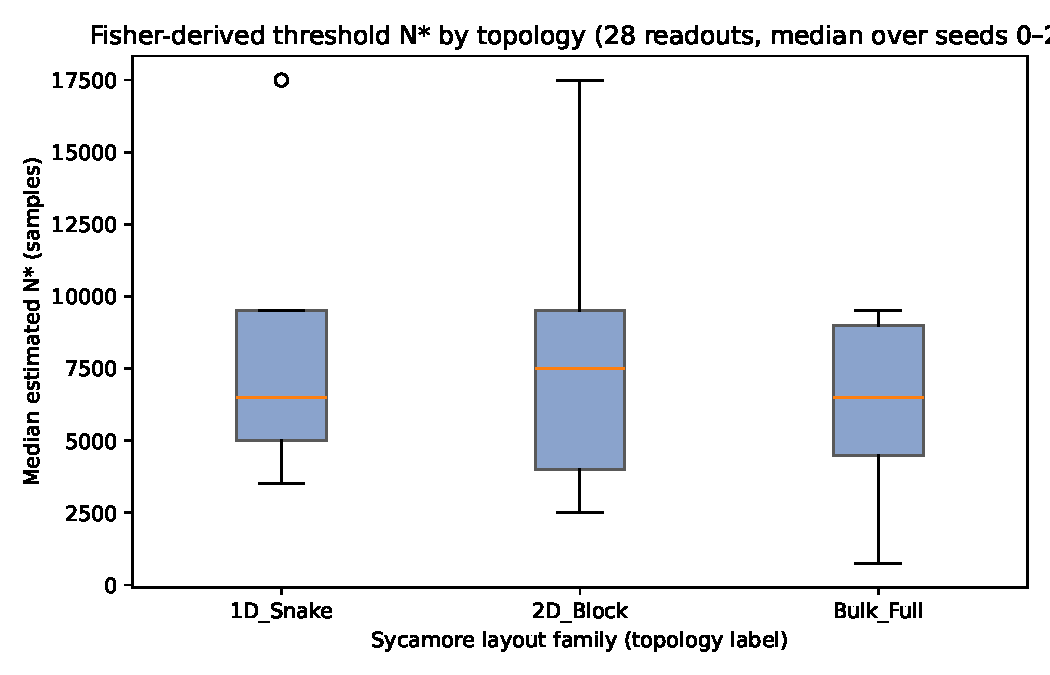
\includegraphics[width=0.92\linewidth]{fig01_median_Nstar_by_topology.pdf}
\caption{Fisher-derived threshold $N^\star$ by Sycamore topology family. Boxplots: median and IQR across readouts within each family, aggregated over seeds 0--2.}
\label{fig:topo}
\end{figure}

\textbf{3.2 Fisher trace dynamics.} Figure~2 shows representative Fisher trace curves versus $N$ for three configurations (seed~0). The trace rises, peaks near $N^\star$, then declines on the grid---a pattern discussed below as suggestive of a specialization peak, with the caveat that the grid is discrete.

\begin{figure}[htbp]
\centering
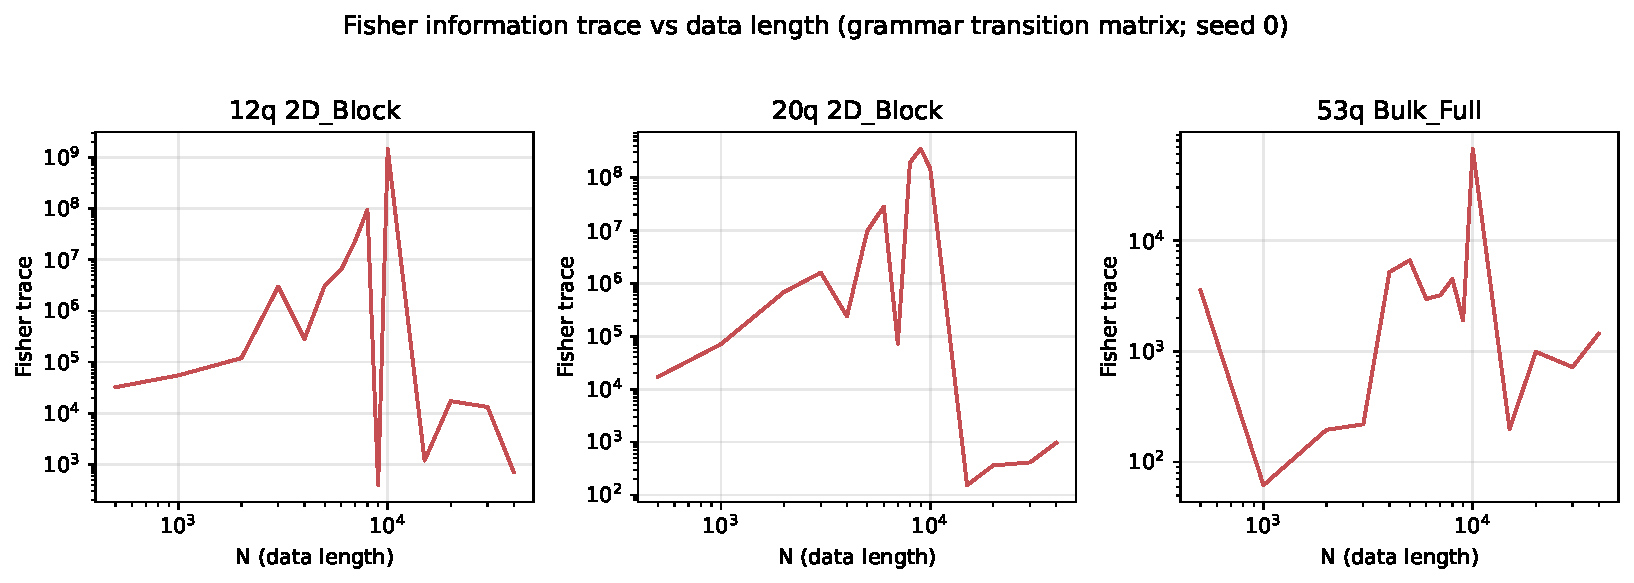
\includegraphics[width=\linewidth]{fig02_fisher_trace_vs_N_examples_seed0.pdf}
\caption{Fisher information trace vs.\ data length $N$ for three representative readouts (seed~0). Log--log axes.}
\label{fig:trace}
\end{figure}

\textbf{3.3 Per-readout thresholds and seed stability.} Figure~3 reports median $N^\star$ and IQR for all 28 readouts. Several configurations exhibit large IQR (e.g., some mid-$q$ layouts); others are stable across seeds.

\begin{figure}[htbp]
\centering
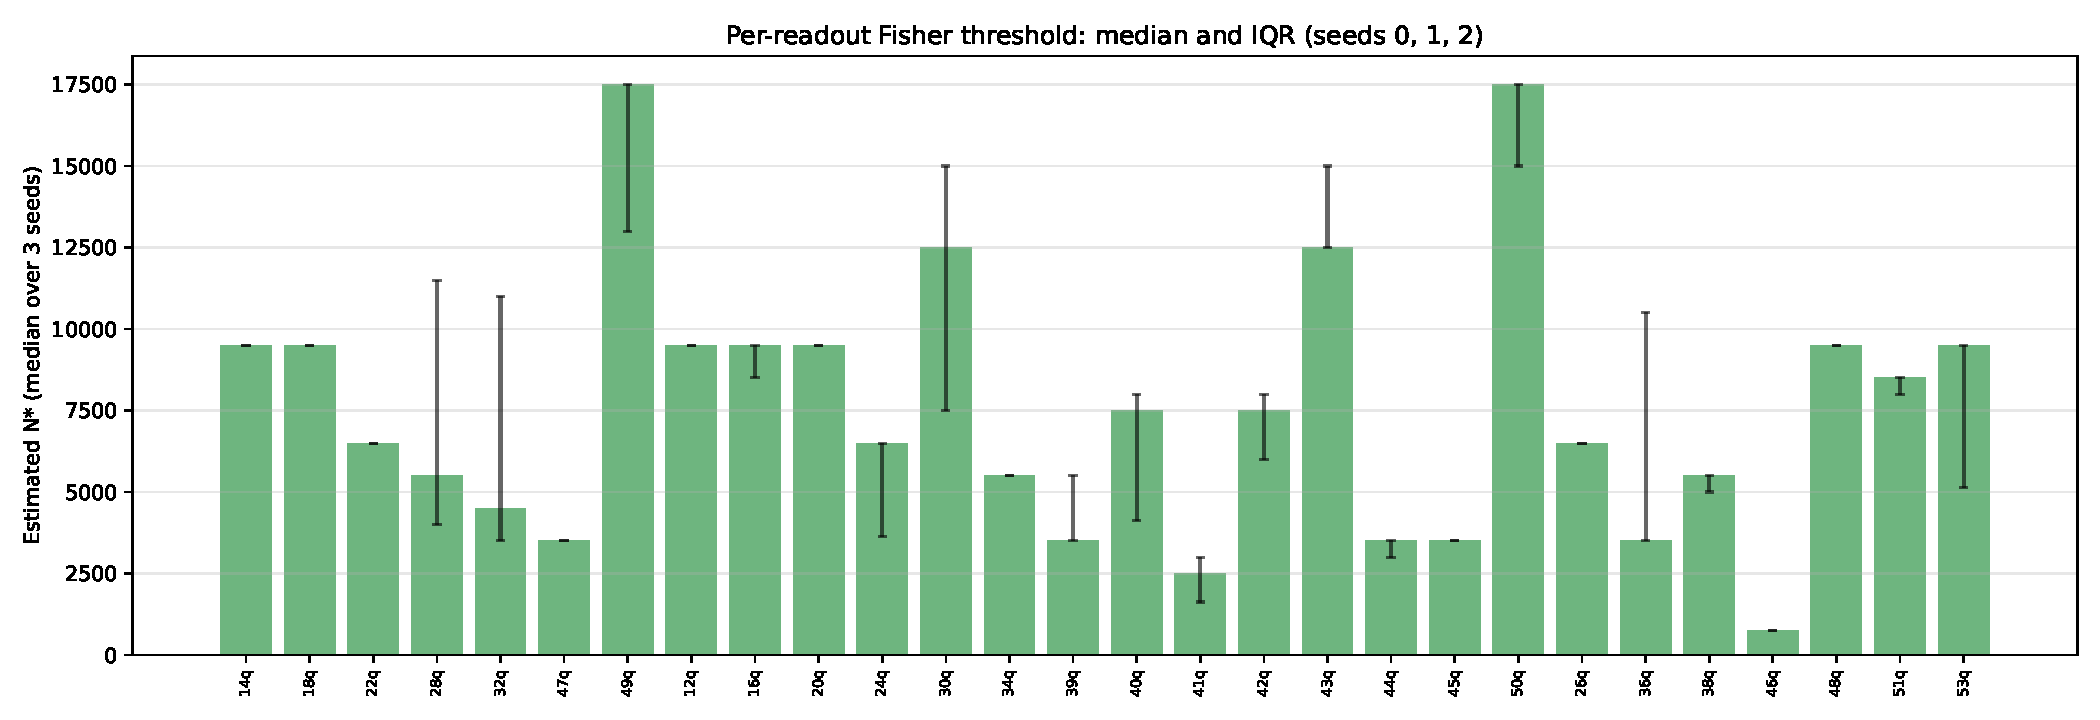
\includegraphics[width=\linewidth]{fig03_median_Nstar_with_IQR_all_readouts.pdf}
\caption{Per-readout Fisher threshold: median $N^\star$ over three seeds with IQR error bars (all 28 configurations).}
\label{fig:readouts}
\end{figure}

\vspace{0.5em}
\textbf{4.\ Discussion}

The Fisher analysis provides a continuous perspective on the data-length phenomenon reported in the classification study. Median Fisher peaks in the $\sim$6{,}500--7{,}500 range are broadly aligned with the $\sim$8{,}000-point classification regime; exact agreement is not required because the two metrics differ (accuracy vs.\ trace peak).

The overlap of topology-wise boxplots supports the view that the scale $N^\star$ is tied to learning dynamics and aggregate noise statistics on Sycamore, while topology-specific structure may appear more clearly in the \emph{shape} of $T$ than in a single scalar threshold.

\vspace{0.5em}
\textbf{5.\ Cross-platform context}

Parallel Fisher threshold analyses were performed on IBM Quantum hardware (e.g.\ Marrakesh, Torino; multiple circuit types; 40{,}960 shots). IBM thresholds vary strongly by circuit family (e.g.\ Hadamard/layers vs.\ GHZ vs.\ identity), unlike the relatively compressed Sycamore band. This contrast reflects different experimental designs: IBM families differ in output statistics; Sycamore layouts differ more subtly in noise correlations.

A phenomenological \textbf{threshold transfer} model was fit on pooled IBM and Sycamore rows. The improved pipeline uses Ridge regression on $\log(N^\star\sqrt{Q})$ with backend and regime indicators, winsorization, and stratified cross-validation; predictions are mapped back to $N$, and metrics are reported in $\log N$ space for observed vs.\ predicted $N^\star$. The full-sample Ridge fit yields $R^2 \approx 0.62$ in that evaluation space. For comparison, ordinary least squares on $\log N^\star$ with the same linear design (intercept, $\log Q$, backend and regime dummies) yields in-sample $R^2 \approx 0.63$ on its training target---so the Ridge value is \emph{not} ``lower because OLS reached 0.85''; the two $R^2$ definitions and targets differ. Out-of-sample, mean CV RMSE in $\log N$ is slightly better for Ridge than for the baseline OLS procedure reported alongside the pipeline. Full tables: supplementary CSVs.

\vspace{0.5em}
\textbf{6.\ Limitations}

Thresholds depend on the discrete $N$ grid; finer sampling near the peak would refine $N^\star$. The LSTM is small (hidden 32); larger models may shift the scale. IBM results are contextual: IBM controls did not meet the same stringency as Sycamore controls in the Grammar study; the IBM circuit-label task is not equivalent to blind Sycamore topology recovery.

\vspace{0.5em}
\textbf{7.\ Conclusion}

Fisher information analysis of Grammar Fingerprinting transition matrices yields a robust information scale on the order of thousands of samples on Sycamore, consistent with the Grammar classification data-length threshold. The scale is reproducible across many seeds and readouts; topology boxplots overlap, and formal tests were not required for the exploratory claims here.

\vspace{0.6em}
\textbf{References}

Arute, F., et al.\ (2019). Quantum supremacy using a programmable superconducting processor. \textit{Nature}, 574, 505--510. DOI: \href{https://doi.org/10.1038/s41586-019-1666-5}{10.1038/s41586-019-1666-5}.

Csapl\'ar, D.\ (2026). Grammar Fingerprinting of Quantum Processor Topology via SAX-LSTM Analysis. Zenodo. DOI: \href{https://doi.org/10.5281/zenodo.19158088}{10.5281/zenodo.19158088}.

Ringbauer, M., et al.\ (2018). Multi-time quantum correlations with no spatial analog. \textit{npj Quantum Information}, 4, 37.

Budroni, C., et al.\ (2022). Temporal correlations in the simplest measurement sequences. \textit{Quantum}, 6, 623.

\vspace{0.5em}
\textbf{Data and code availability}

Sycamore readout data: Dryad DOI \href{https://doi.org/10.5061/dryad.k6t1rj8}{10.5061/dryad.k6t1rj8}. Grammar Fingerprinting code and validation results: Zenodo \href{https://doi.org/10.5281/zenodo.19158088}{10.5281/zenodo.19158088}.

\textbf{Fisher continuation (this work):} code, CSV results, figure PDFs/PNGs, and this preprint are deposited as a separate Zenodo record (DOI issued on publication). A related identifier links this deposit to the Grammar Zenodo record above. Figure source files: \texttt{results/fisher\_figures/} in the development repository.

Code repository: \href{https://github.com/csaplard/QuantumCircuit_Grammar_Research}{\texttt{csaplard/QuantumCircuit\_Grammar\_Research}} (confirm branch/release before citation).

\end{document}
